%% The following is a directive for TeXShop to indicate the main file
%%!TEX root =../diss.tex

\chapter{Introduction}
\label{ch:Introduction}

\section{Cancer}

Some facts about prevalence of cancer and poor outcomes, high toxicity to motivate this work.

\subsection{Current therapies}

Numerous advancements in chemotherapies over the past decade have sparked an urgent clinical need for non invasive methods to assess treatment efficacy.
There is a knowledge gap in the use and synergistic combinations of therapies, and many treatment regimens expose patients to higher toxicity than necessary.
Despite known extremes in patient response to treatment - even in cancers of the same type and grade - doses are generally prescribed by success rates of trials in patient populations exhibiting similar disease manifestations.
Each class of drugs has unique modes of action and still, there are no reliable and reproducible methods to assess synergistic benefits of combined therapy regimens~\cite{Zhang:2008ie}.
Traditionally, a prominent measure of treatment response has been to track tumour shrinkage following treatment~\cite{Tuma:2006hx}.
However, it has been shown that tumour shrinkage can take weeks and sometimes even months to manifest~\cite{Brindle:2008jt} and in some cases may not occur at all~\cite{Kitzen:2008un}.
For instance, anti-angiogenic agents typically arrest tumour growth by disrupting existing vasculature or inhibiting new vessel growth.
Despite positive effect, these agents may not necessarily lead to tumour shrinkage.
This mode of drug action is better characterized by assessing tumour vascular function rather than gross changes in physical size.
Development of quantitative and non-invasive methods to assess tumours following therapy continues to be a burgeoning field.Furthermore, there is an urgent need in the drug development and testing community as drugs that fail in the late stages of clinical trials have led to an astronomical rise in the cost of developing drugs.
Lack of any patient stratification techniques to identify potential responders from non-responders is a key reason that drugs fail.
For instance clinical trials targeting hypoxia- a key target for both chemotherapy to improve drug delivery and radiotherapy to increase radiosensitivity - have been conducted without patient selection or stratification based on pre-treatment tumour hypoxia status and therefore include patients with different hypoxic fractions~\cite{Overgaard:2011ji}.
This is at least partially due to an absence of validated methods that can accurately assess the hypoxia status of tumours.The benefits of developing early, non-invasive measures of treatment efficacy are clear for both patients and health care systems.
For patients, if a standard treatment regimen is prescribed and deemed ineffective early, the treatment can be altered and patients can directly benefit from personalized care.
Similarly, with improved patient stratification using non-invasive gross assessments of the tumour status, these patients can avoid receiving potentially ineffective and expensive therapies leading us one stop closer to personalized medicine.
However, the choice of appropriate biomarkers for particular targets remains elusive. 

\subsection{Cancer Biomarkers and targets} There has been considerable interest in predictive biomarkers for early assessment.
Several candidates have appeared and disappeared but in 2000, a seminal paper catalogued a vast array of cancer cell genotypes into ``six essential alterations in cell physiology that collectively dictate malignant growth in tumours''~\cite{Hanahan:2000wo} (figure~\ref{cancerHallmarks}): 1) self-sufficiency in growth signals, 2) insensitivity to growth-inhibitory signals, 3) evasion of programmed cell death, 4) limitless replicative potential, 5) sustained angiogenesis and, 6) tissue invasion and metastasis~\cite{Hanahan:2000wo}.
In 2011, taking into account the progress made over a decade, the framework expanded to inculde four more hallmarks for the next generation~\cite{Hanahan:2011gu}.
Angiogenesis, the 5th hallmark is particularly suitable for consideration in non-invasive imaging techniques, particularly MRI. 

\begin{figure}[htbp]   
 \begin{center}  
 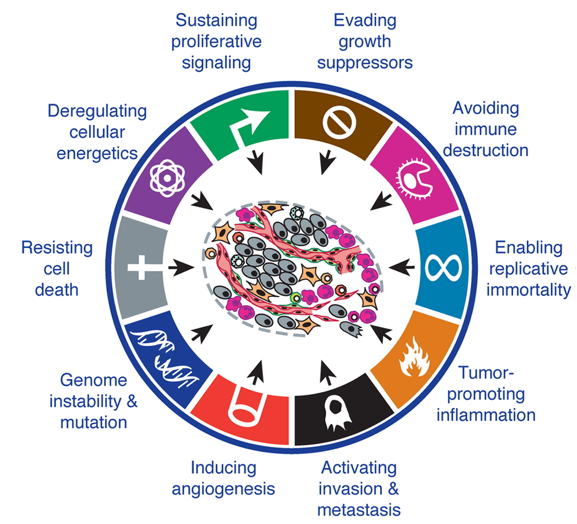
\includegraphics[width=4in]{intro/./intro-images/cancerHallmarks.png}
 \caption{Graphical illustration of the hallmarks of cancer; many of these targets are inaccessible to non-invasive imaging. Figure from the Hanahan group~\cite{Hanahan:2011gu}.}  
 \label{cancerHallmarks}  
 \end{center}
\end{figure}

Angiogenesis, or the formation of new blood vessels from pre-existing ones is a normal and vital process in the body tightly regulated by various cell signalling pathways and growth factors.
In tumours, angiogenesis is a critical step in the growth and spread of tumours as new blood vessels are recruited from the existing vascular network to promote rapidly accelerated and abnormal tumour growth~\cite{Folkman:1990ud}.
Normally, this process is regulated by several angiogenic and antiangiogenic factors such as $\alpha \beta$ integrin, vascular endothelial growth factor (VEGF) and fibroblast growth factor (FGF)~\cite{Laking:2006ij}.
In tumours however, this process is completely deregulated (figure~\ref{tumourVasculature}) and excess production of growth factors from rapidly proliferating tumour cells leads to a drastic increase in vasculogenesis.
These newly formed vessels are unstable and must mature with the addition of pericytes, cells that surround the endothelium providing structural support.
Pericytes are often malformed and poorly distributed in solid tumours contributing to a dysfunctional vascular network.
Vessel growth patterns in tumours are generally accepted to be abnormal with a defective and leaky endothelium~\cite{McDonald:2002ut}.
Irregular diameters of tumour vessels, abnormal branching patterns and leaky vessel walls all contribute to an increase in vessel permeability.
It is estimated that a single hole larger than 0.5$\mu$m in diameter would alter the permeability of that vessel significantly enough to result in solute extravasation to be limited by blood flow~\cite{McDonald:2002ut}.
Disorganized and inefficient blood flow also limits the delivery of macromolecules, such as chemotherapeutic agents via the blood.
Poor perfusion in the tumour due to a disorganized vascular network impairs the delivery of systemic drugs to the whole tumour and ultimately, reduces efficacy. 

%\begin{wrapfigure}{L}{0.65\textwidth} 
\begin{figure}  
 \begin{center}  
 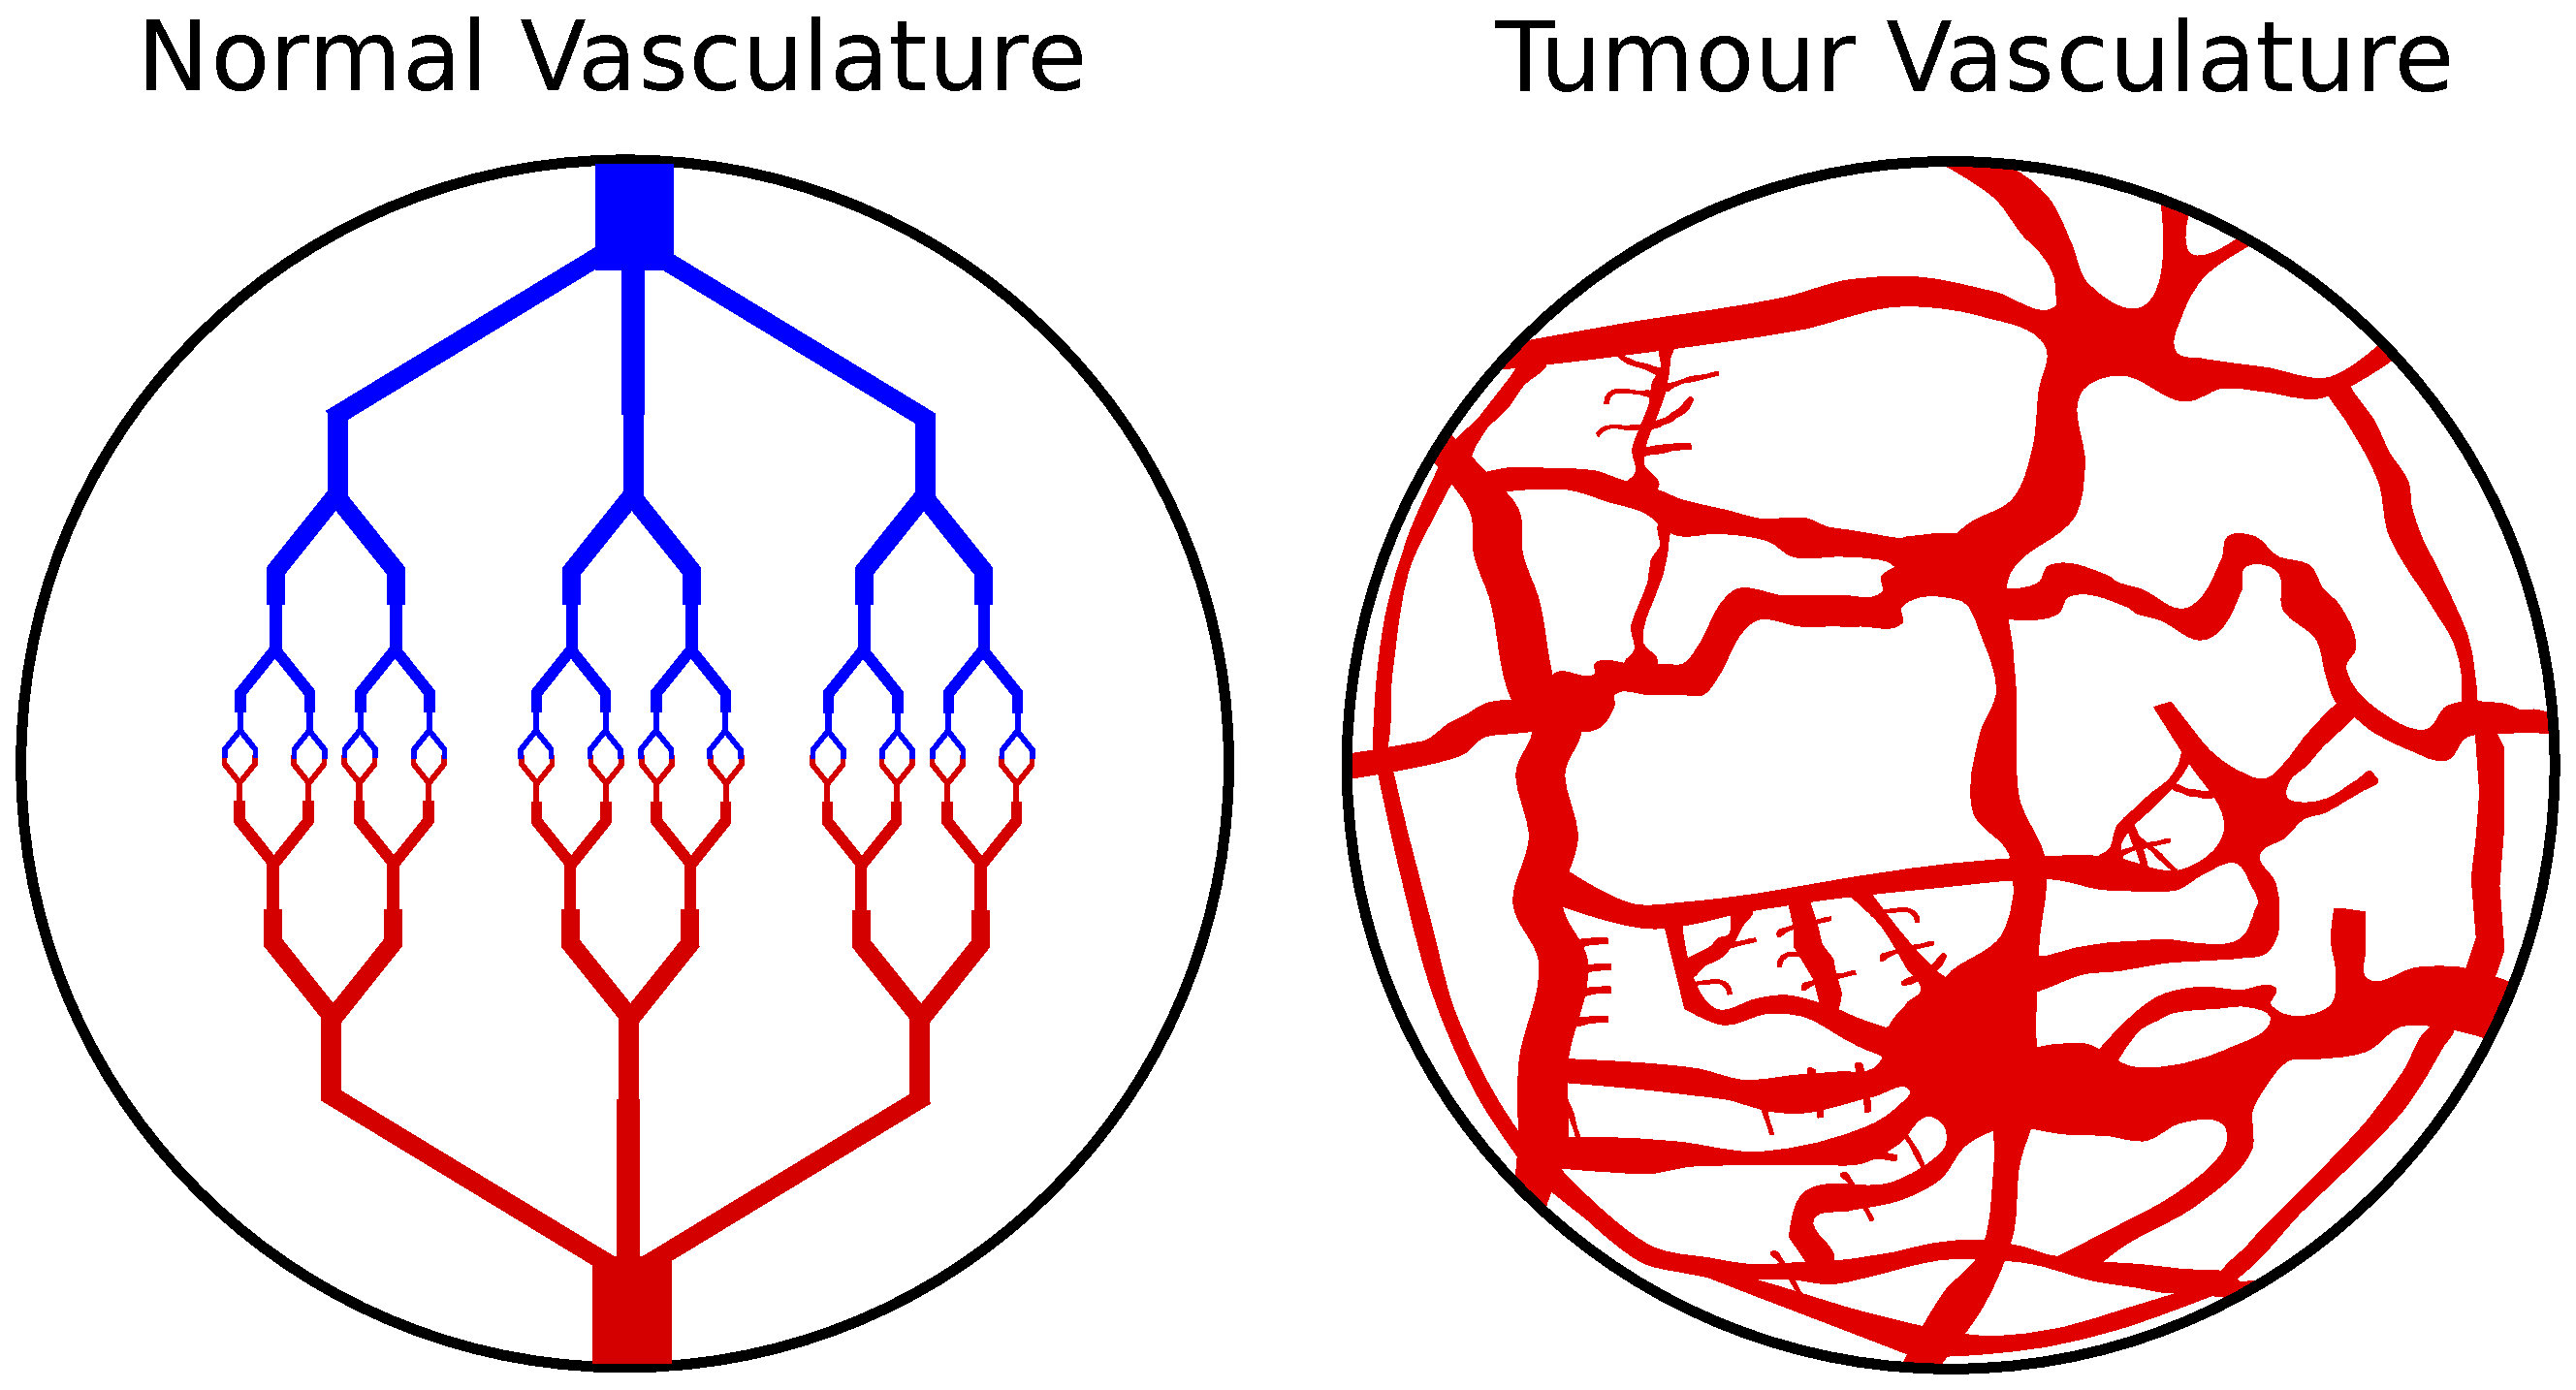
\includegraphics[width=4in]{intro/./intro-images/tumourVasculature.pdf}
 \caption{Schematic of the normal tissue (left) and tumour (right) vasculature network. 
 Note the hierarchical structure of oxygenated blood (red) passing through the arteries, arterioles, and deoxygenated blood leaving via the venules, veins. 
 In tumours, this structure is severely compromised and often, no clear flow patterns can be distinguished with many vessels ending in dead ends or looping back onto feeding vessels.}
 \label{tumourVasculature}
 \end{center}
\end{figure}

Several strategies have been proposed to maximize cell kill, including the combination of different therapies (such as radiotherapy and chemotherapy) and agents that ``normalize'' the tumour vasculature and prime them for receiving chemotherapies~\cite{Jain:2005gk}.
Tumour angiogenesis is extremely important in tumour growth, progression and metastasis and is a promising target for novel therapies~\cite{Miles:2000wq}.
For instance, ``measuring'' tumour angiogenesis has the potential to serve as a highly predictive prognostic marker for disease outcome and treatment.
Histology remains the gold standard for angiogenesis detection (microvessel density) but has several critical limitations.
Histology requires biopsy samples and patient comfort aside, biopsies only sample a small fraction of the potentially affected organ.
The lack of functional information from biopsies as well as the practical challenges of obtaining longitudinal biopsy samples make non-invasive imaging a promising technique to complement and potentially reduce unneeded biopsies.

\subsection{Need for non-invasive imaging}
Non-invasive imaging methods are proving indispensable for studying angiogenesis \emph{in vivo}~\cite{McDonald:2003cm} as they provide researchers with quantitative information about blood flow, vascular permeability, vessel density, vessel function and blood volume.
 Imaging modalities such as computed tomography (CT), magnetic resonance imaging (MRI), positron emission tomography (PET), single photon emission computed tomography (SPECT) and ultrasound (US), have all been proposed for studying angiogenesis~\cite{Laking:2006}.
Each modality is optimal for probing a particular aspect of biomarkers. To study angiogenesis and its effects on tumour growth and treatment response, the tumour environment needs to be probed using tools that assess both the interstitial tumour volume as well as the tumour vasculature.
Nuclear medicine techniques such as PET and SPECT employ radiotracers that can be measured at picomolar concentrations but at a significantly lower spatial resolution.
DCE-MRI and DCE-CT offer similar perfusion measurements (rate of leakage and leakage space) as both rely on the administration of a contrast agent that diffuses from the vasculature.
DCE-CT is advantageous as it has a direct linear relationship between the contrast agent concentration and the image intensity (attenuation numbers, given by Houndsfield Units)~\cite{Cuenod:2006jy}.
The disadvantage of CT however is that it requires ionizing radiation and iodinated contrast agents used in CT have been shown to have lower safety profiles compared to MR contrast agents~\cite{Hasebroock:2009hw}.
MRI can also be used to measure additional information such as diffusion, tissue oxygenation, spectroscopy, chemical exchange and magnetization transfer. 
In this thesis, several techniques will be explored in a bid to improve our understanding of the tumour microenvironment.

\section{Magnetic Resonance Imaging}
\subsection{T$_1$}
\subsection{T$_2^*$}

\subsection{Contrast mechanisms}
Split into two groups - there are others, but this is what's relevant for this thesis.

Talk about relaxivity and tumbling, water protons.

\subsubsection{Low-MW Agents}
\begin{itemize}
\item Gd-DTPA
\item Modeling (Tofts)
\end{itemize}

\subsubsection{High-MW Agents}
\begin{itemize}
\item Dextran based agents
\item Relaxivity
\end{itemize}

\subsection{Oxygen as a contrast agent}

\section{Thesis structure}

\begin{enumerate}
\item Introduction to Cancer and imaging
\item [New contrast agent using HPG] MRI and histology of vascular function in xenografts using HPG - using a high MW contrast agent to explore vascular function
\item [Application of new agent HPG] Heterogeneous distribution of trastuzumab in HER2-positive xenografts and metastases: role of the tumour microenvironment 
\end{enumerate}
